\documentclass[aspectratio=169,10pt]{beamer}

\usetheme{Madrid}
\usecolortheme{seahorse}

%\usepackage[utf-8]{inputenc}
\usepackage{amsmath}
\usepackage{amssymb}
\usepackage{amsfonts}
\usepackage{graphics}
\usepackage{listings}
\usepackage{xcolor}
\usepackage{cancel}
\usepackage{tikz}

% Define graphics path
\graphicspath{{figures/}}

% Listings configuration for Python
\lstset{
  language=Python,
  basicstyle=\ttfamily\scriptsize,
  commentstyle=\color{green!50!black}\itshape,
  keywordstyle=\color{blue}\bfseries,
  stringstyle=\color{red},
  showstringspaces=false,
  breaklines=true,
  numbers=left,
  numberstyle=\tiny\color{gray},
  frame=single,
  backgroundcolor=\color{gray!10},
  tabsize=2
}

% Theorem environments
\newtheorem{prop}{Proposition}
\newtheorem{thm}{Theorem}
\newtheorem{dfn}{Definition}
\newtheorem{cor}{Corollary}
\newtheorem{rmk}{Remark}
\newtheorem{exmp}{Example}

% Mathematical operators
\DeclareMathOperator{\dom}{dom}
\DeclareMathOperator{\prox}{prox}
\DeclareMathOperator{\pav}{pav}
\DeclareMathOperator{\Prox}{Prox}

\setbeamertemplate{footline}[frame number]
\setbeamertemplate{navigation symbols}{}

\title[Chapter 14: Further Conjugation]{Chapter 14: Further Conjugation Results}
\subtitle{Convex Analysis and Monotone Operator Theory in Hilbert Spaces}
\author[Bauschke \& Combettes]{H.H. Bauschke and P.L. Combettes}
\date{2e, 2017}

\begin{document}

\frame{\titlepage}

% ━━━━━━━━━━━━━━━━━━━━━━━━━━━━━━━━━━━━━━━━━━━━━━━━━━━━━━━━━━━━━━━━━━━━━━━━━━━

\section{Strongly Convex Conjugates}

\begin{frame}{14.1: Strongly Convex Conjugates}
  \vspace{-0.3cm}

  Key question: When does the conjugate of a function relate to strong convexity?

  \begin{prop}[14.2]
    Let $f: \mathcal{H} \to \mathbb{R} \cup \{+\infty\}$ be continuous and convex,
    let $\gamma \in \mathbb{R}_{++}$, and set $q = (1/2)\|\cdot\|^2$. Then:
    \begin{enumerate}
      \item[(i)] $f^* - \gamma^{-1}q$ is convex, i.e., $f^*$ is $\gamma^{-1}$-strongly convex.
      \item[(ii)] $\gamma q - f$ is convex.
    \end{enumerate}
  \end{prop}

  \vspace{0.3cm}

  \textbf{Key insight:} Strong convexity of $f^*$ is equivalent to $\gamma q - f$ being convex.
\end{frame}

\begin{frame}{Strongly Convex Conjugates (cont'd)}
  \vspace{-0.3cm}

  \begin{thm}[14.3]
    Let $f \in \Gamma_0(\mathcal{H})$ and $\gamma \in \mathbb{R}_{++}$. Set $q = (1/2)\|\cdot\|^2$. Then:
    \begin{enumerate}
      \item[(i)] $\gamma^{-1}q = f \square (\gamma^{-1}q) + (f^* \square (\gamma q)) \circ \gamma^{-1}\text{Id}$
      \item[(ii)] $\text{Id} = \Prox_f + \gamma\Prox_{f^*/\gamma} \circ \gamma^{-1}\text{Id}$
      \item[(iii)] For $x \in \mathcal{H}$:
        \[
          f(\Prox_f x) + f^*(\Prox_{f^*/\gamma}(x/\gamma)) = \langle \Prox_f x \mid \Prox_{f^*/\gamma}(x/\gamma) \rangle
        \]
    \end{enumerate}
  \end{thm}

  \vspace{0.2cm}

  where $\square$ denotes infimal convolution (Definition 12.34).
\end{frame}

\begin{frame}{Remark 14.4: Moreau's Decomposition}
  \vspace{-0.3cm}

  When $f = \iota_K$ (indicator of closed convex cone $K$) with $q = (1/2)\|\cdot\|^2$:

  \[
    (f \square q) + (f^* \square q) = q \quad \text{and} \quad \Prox_f + \Prox_{f^*} = \text{Id}
  \]

  This recovers \textbf{Moreau's conical decomposition} (Theorem 6.30).

  \vspace{0.3cm}

  \begin{exmp}[14.5]
    For $f(x) = \rho \|x\|$ (soft threshold function):
    \begin{itemize}
      \item $f^* = \iota_{B(0;\rho)}$ (indicator of ball)
      \item $\Prox_f x = \begin{cases}
        \left(1 - \rho/\|x\|\right) x & \text{if } \|x\| > \rho \\
        0 & \text{if } \|x\| \le \rho
      \end{cases}$ (soft thresholder)
      \item $^{\gamma}f(x) = \begin{cases}
        \rho\|x\| - \rho^2/2 & \text{if } \|x\| > \rho \\
        \|x\|^2/2 & \text{if } \|x\| \le \rho
      \end{cases}$ (Huber function)
    \end{itemize}
  \end{exmp}
\end{frame}

\begin{frame}{Example 14.5 Visualization}
  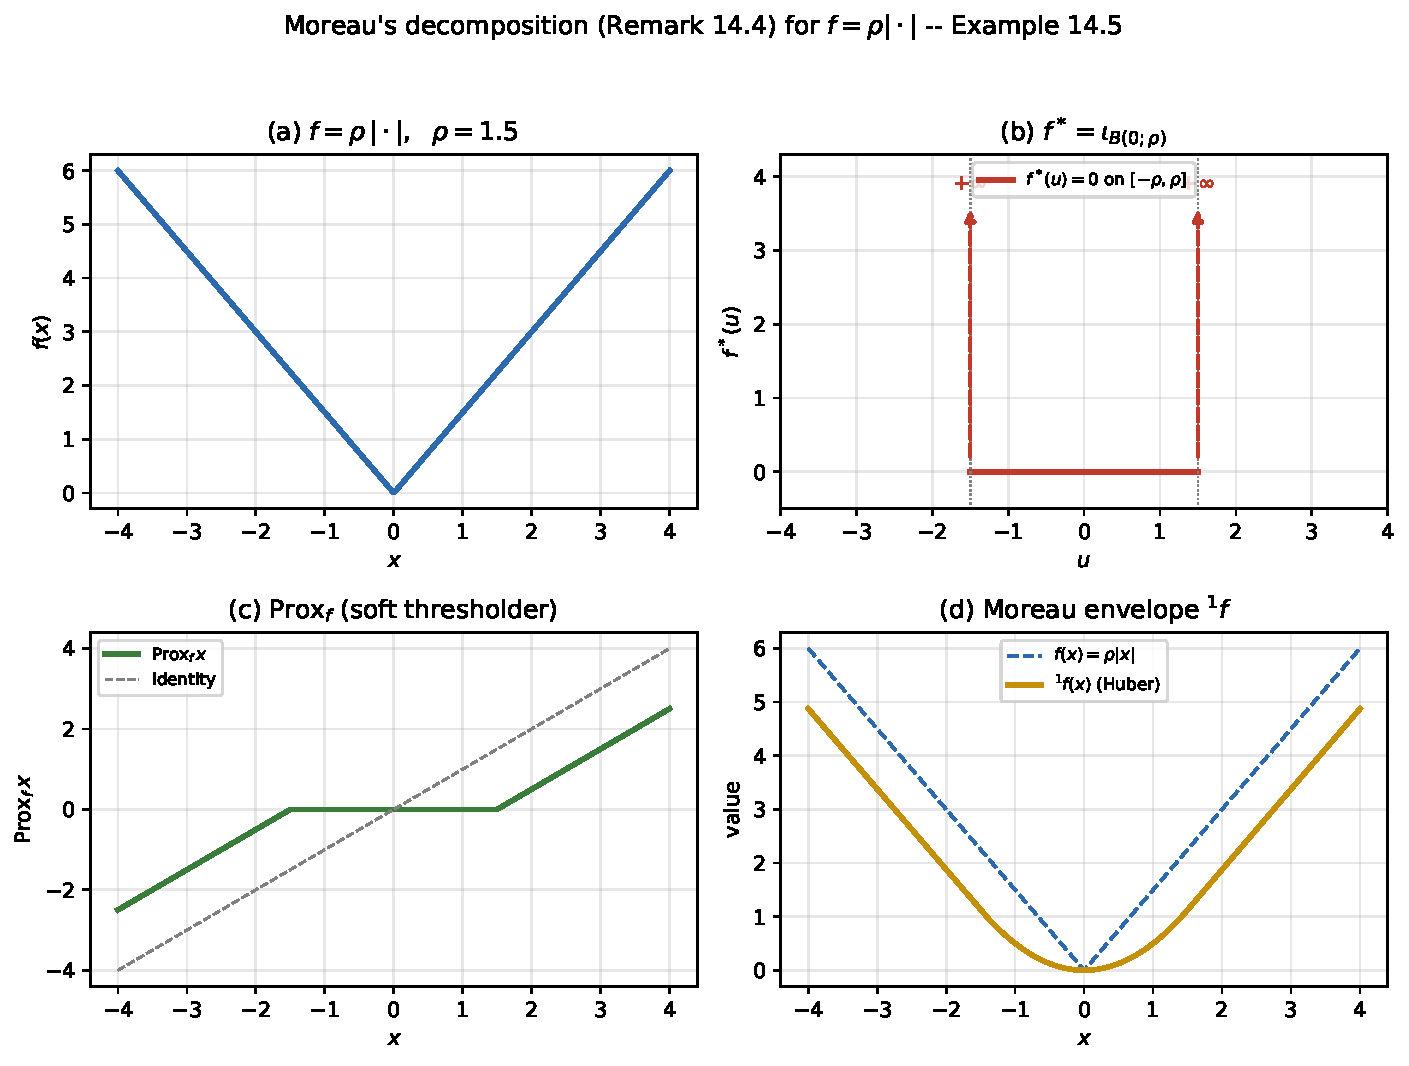
\includegraphics[width=0.95\textwidth]{fig_moreau_decomposition.pdf}
\end{frame}

% ━━━━━━━━━━━━━━━━━━━━━━━━━━━━━━━━━━━━━━━━━━━━━━━━━━━━━━━━━━━━━━━━━━━━━━━━━━━

\section{Proximal Average}

\begin{frame}{14.2: Proximal Average}
  \vspace{-0.3cm}

  \begin{dfn}[14.6]
    Let $f, g \in \Gamma_0(\mathcal{H})$. The \textbf{proximal average} of $f$ and $g$ is:
    \[
      \pav(f,g) : \mathcal{H} \to \mathbb{R} \cup \{+\infty\}, \quad
      x \mapsto \frac{1}{2}\inf_{(y,z) \in \mathcal{H} \times \mathcal{H}, \, y+z=2x}
      \left( f(y) + g(z) + \frac{1}{4}\|y-z\|^2 \right)
    \]
  \end{dfn}

  \vspace{0.2cm}

  \begin{prop}[14.7]
    Set $L(y,z) = (y+z)/2$ and $F(y,z) = \frac{1}{2}f(y) + \frac{1}{2}g(z) + \frac{1}{8}\|y-z\|^2$.
    Then for $f, g \in \Gamma_0(\mathcal{H})$:
    \begin{enumerate}
      \item[(i)] $\pav(f,g) = L \triangleright F$
      \item[(ii)] $\pav(f,g) = L \triangleright F$
      \item[(iii)] $\dom \pav(f,g) = \frac{1}{2}\dom f + \frac{1}{2}\dom g$
      \item[(iv)] $\pav(f,g)$ is a proper convex function
    \end{enumerate}
  \end{prop}
\end{frame}

\begin{frame}{Proximal Average Properties}
  \vspace{-0.3cm}

  \begin{cor}[14.8]
    Let $f, g \in \Gamma_0(\mathcal{H})$ and $q = (1/2)\|\cdot\|^2$. Then:
    \begin{enumerate}
      \item[(i)] $\pav(f,g) \in \Gamma_0(\mathcal{H})$
      \item[(ii)] $(\pav(f,g))^* = \pav(f^*, g^*)$ (conjugate of proximal average)
      \item[(iii)] $\pav(f,g) \square q = \frac{1}{2}(f \square q) + \frac{1}{2}(g \square q)$
      \item[(iv)] $\Prox_{\pav(f,g)} = \frac{1}{2}\Prox_f + \frac{1}{2}\Prox_g$
    \end{enumerate}
  \end{cor}

  \vspace{0.3cm}

  \textbf{Remark:} The proximal average is self-dual (part ii) and satisfies a
  beautiful sandwich property (Proposition 14.9).
\end{frame}

\begin{frame}{Proximal Average Bounds}
  \vspace{-0.3cm}

  \begin{prop}[14.9]
    Let $f, g \in \Gamma_0(\mathcal{H})$. Then:
    \[
      \left( \frac{1}{2}f^* + \frac{1}{2}g^* \right)^* \le \pav(f,g) \le \frac{1}{2}f + \frac{1}{2}g
    \]
  \end{prop}

  \begin{prop}[14.10]
    Let $F, G \in \Gamma_0(\mathcal{H} \oplus \mathcal{H})$. Then:
    \[
      (\pav(F, G))^{\top} = \pav(F^{\top}, G^{\top})
    \]
    where $F^{\top}(y,z) = F(z,y)$ is the transpose.
  \end{prop}
\end{frame}

\begin{frame}{Proximal Average Visualization}
  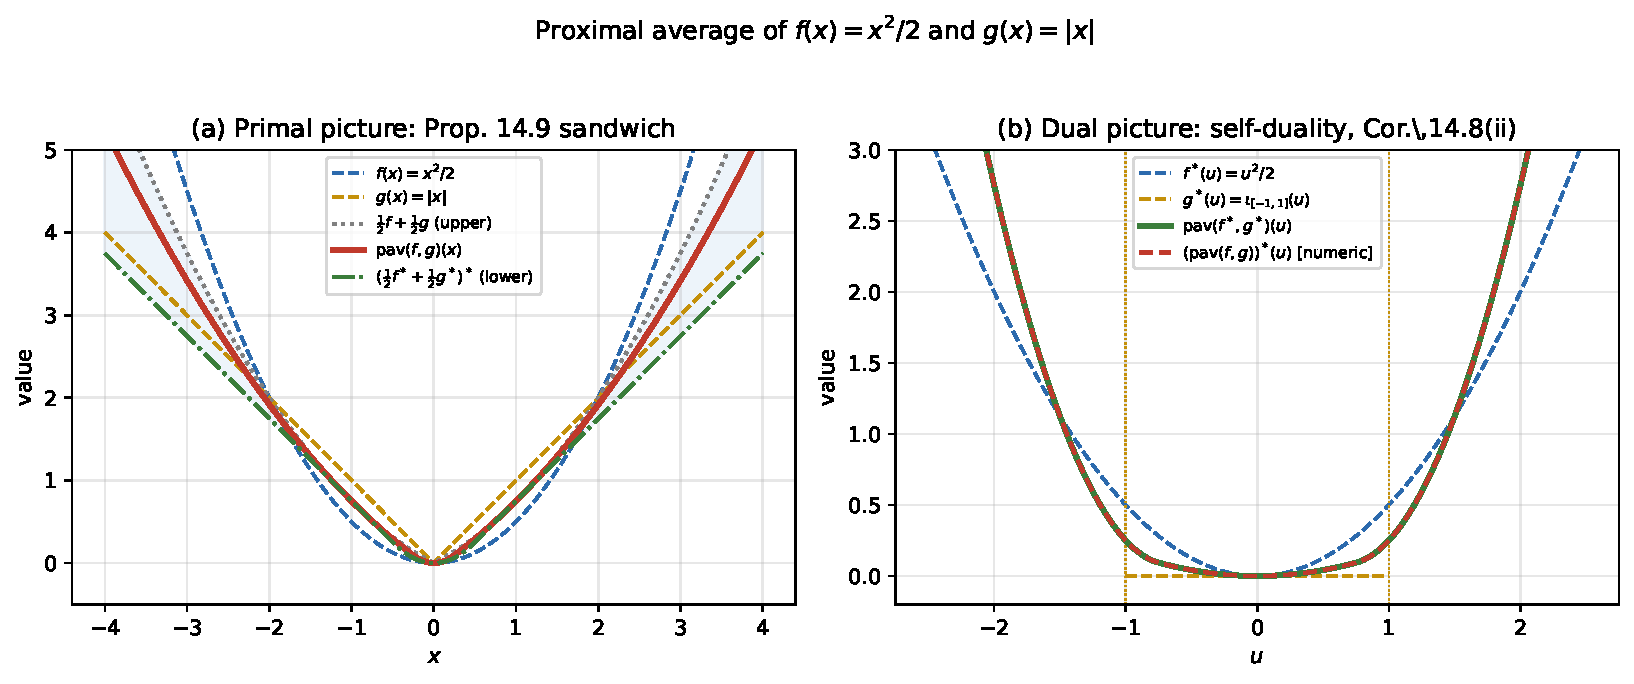
\includegraphics[width=0.95\textwidth]{fig_proximal_average.pdf}
\end{frame}

% ━━━━━━━━━━━━━━━━━━━━━━━━━━━━━━━━━━━━━━━━━━━━━━━━━━━━━━━━━━━━━━━━━━━━━━━━━━━

\section{Positively Homogeneous Functions}

\begin{frame}{14.3: Positively Homogeneous Functions}
  \vspace{-0.3cm}

  \begin{prop}[14.11]
    Let $f: \mathcal{H} \to \mathbb{R} \cup \{+\infty\}$ and set
    $C = \{u \in \mathcal{H} \mid (\forall x \in \mathcal{H}) \langle x \mid u \rangle \le f(x)\}$.

    Then the following are equivalent:
    \begin{enumerate}
      \item[(i)] $f$ is positively homogeneous and $f \in \Gamma_0(\mathcal{H})$
      \item[(ii)] $f = \sigma_C$ and $C$ is nonempty, closed, and convex
      \item[(iii)] $f$ is the support function of a nonempty closed convex subset of $\mathcal{H}$
    \end{enumerate}
  \end{prop}

  \vspace{0.2cm}

  \textbf{Key insight:} Positively homogeneous convex functions are exactly support functions
  of closed convex sets.
\end{frame}

\begin{frame}{Support Function and Minkowski Gauge}
  \vspace{-0.3cm}

  \begin{prop}[14.12]
    Let $C$ be a convex subset of $\mathcal{H}$ such that $0 \in C$. Then:
    \[
      m_C^* = \iota_{C^{\circ}}
    \]
    where $m_C$ is the Minkowski gauge of $C$.
  \end{prop}

  \vspace{0.2cm}

  \begin{cor}[14.13]
    Let $C$ be a closed convex subset of $\mathcal{H}$ such that $0 \in C$. Then:
    \begin{enumerate}
      \item[(i)] $C = \text{lev}_{\le 1} m_C$
      \item[(ii)] If $0 \in \text{int} C$, then $\text{int} C = \text{lev}_{<1} m_C$
    \end{enumerate}
  \end{cor}
\end{frame}

\begin{frame}{Positively Homogeneous Functions Visualization}
  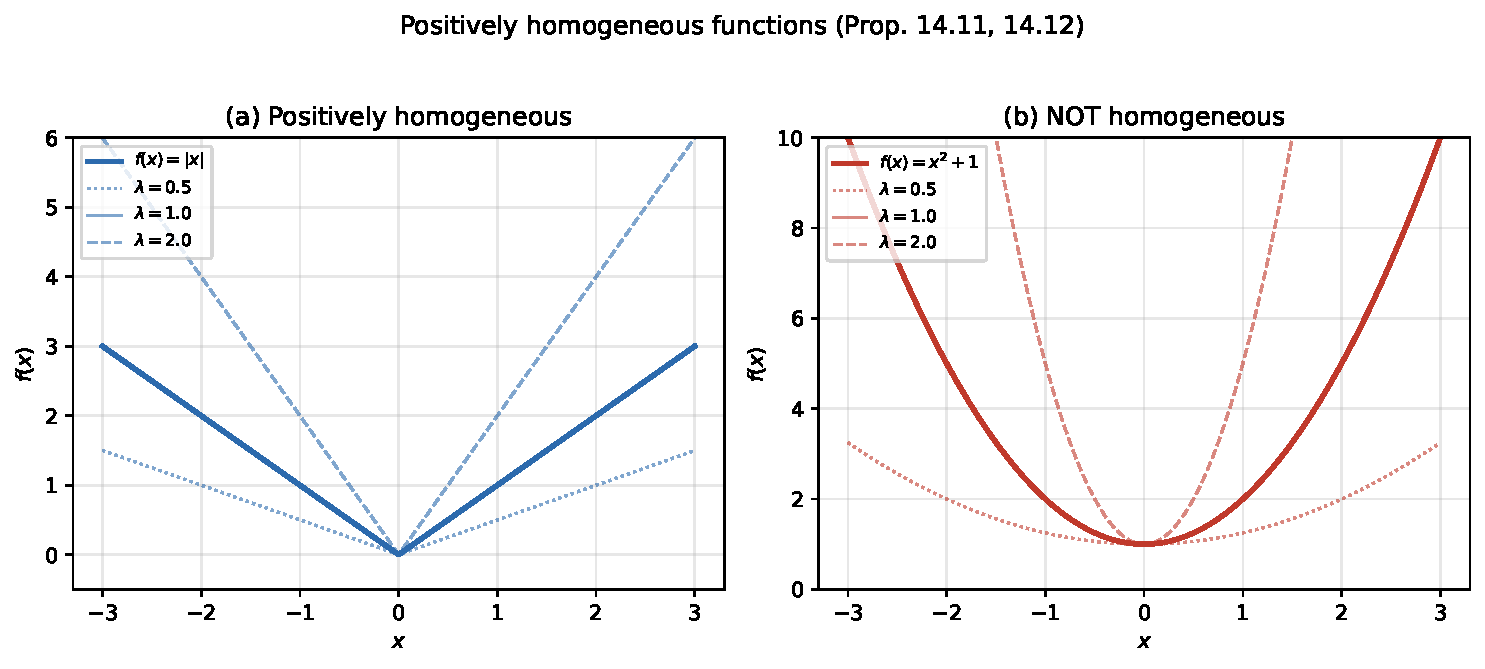
\includegraphics[width=0.95\textwidth]{fig_positively_homogeneous.pdf}
\end{frame}

% ━━━━━━━━━━━━━━━━━━━━━━━━━━━━━━━━━━━━━━━━━━━━━━━━━━━━━━━━━━━━━━━━━━━━━━━━━━━

\section{Coercivity}

\begin{frame}{14.4: Coercivity}
  \vspace{-0.3cm}

  \begin{prop}[14.14]
    Let $f \in \Gamma_0(\mathcal{H})$, $\alpha \in \mathbb{R}_{++}$, and consider:
    \begin{enumerate}
      \item[(i)] $\liminf_{\|x\| \to +\infty} f(x)/\|x\| > \alpha$
      \item[(ii)] $(\exists \beta \in \mathbb{R})$ $f \ge \alpha \|\cdot\| + \beta$
      \item[(iii)] $(\exists \gamma \in \mathbb{R})$ $f^*|_{B(0,\alpha)} \le \gamma$
      \item[(iv)] $\liminf_{\|x\| \to +\infty} f(x)/\|x\| \ge \alpha$
    \end{enumerate}

    Then $(i) \Rightarrow (ii) \Leftrightarrow (iii) \Rightarrow (iv)$.
  \end{prop}
\end{frame}

\begin{frame}{Characterization of Coercivity}
  \vspace{-0.3cm}

  \begin{prop}[14.15]
    Let $f \in \Gamma_0(\mathcal{H})$. Consider:
    \begin{enumerate}
      \item[(i)] $f$ is supercoercive
      \item[(ii)] $f^*$ is bounded on every bounded subset of $\mathcal{H}$
      \item[(iii)] $\dom f^* = \mathcal{H}$
    \end{enumerate}

    Then $(i) \Leftrightarrow (ii) \Rightarrow (iii)$.
  \end{prop}

  \vspace{0.3cm}

  \begin{thm}[14.16]
    Let $f \in \Gamma_0(\mathcal{H})$. The following are equivalent:
    \begin{enumerate}
      \item[(i)] $f$ is coercive
      \item[(ii)] The lower level sets $(\text{lev}_{\le c} f)_{c \in \mathbb{R}}$ are bounded
      \item[(iii)] $\liminf_{\|x\| \to +\infty} f(x)/\|x\| > 0$
      \item[(iv)-(vi)] [Additional characterizations via subdifferentials]
    \end{enumerate}
  \end{thm}
\end{frame}

\begin{frame}{Moreau-Rockafellar Theorem}
  \vspace{-0.3cm}

  \begin{thm}[14.17: Moreau-Rockafellar]
    Let $f \in \Gamma_0(\mathcal{H})$ and $u \in \mathcal{H}$. Then:
    \[
      f - \langle \cdot \mid u \rangle \text{ is coercive} \quad \Leftrightarrow \quad u \in \text{int} \dom f^*
    \]
  \end{thm}

  \vspace{0.3cm}

  \begin{cor}[14.18]
    Let $f, g \in \Gamma_0(\mathcal{H})$ and suppose $f$ is supercoercive. Then:
    \begin{enumerate}
      \item[(i)] $f \square g$ is coercive if and only if $g$ is coercive
      \item[(ii)] $f \square g$ is supercoercive if and only if $g$ is supercoercive
    \end{enumerate}
  \end{cor}
\end{frame}

\begin{frame}{Coercivity Visualization}
  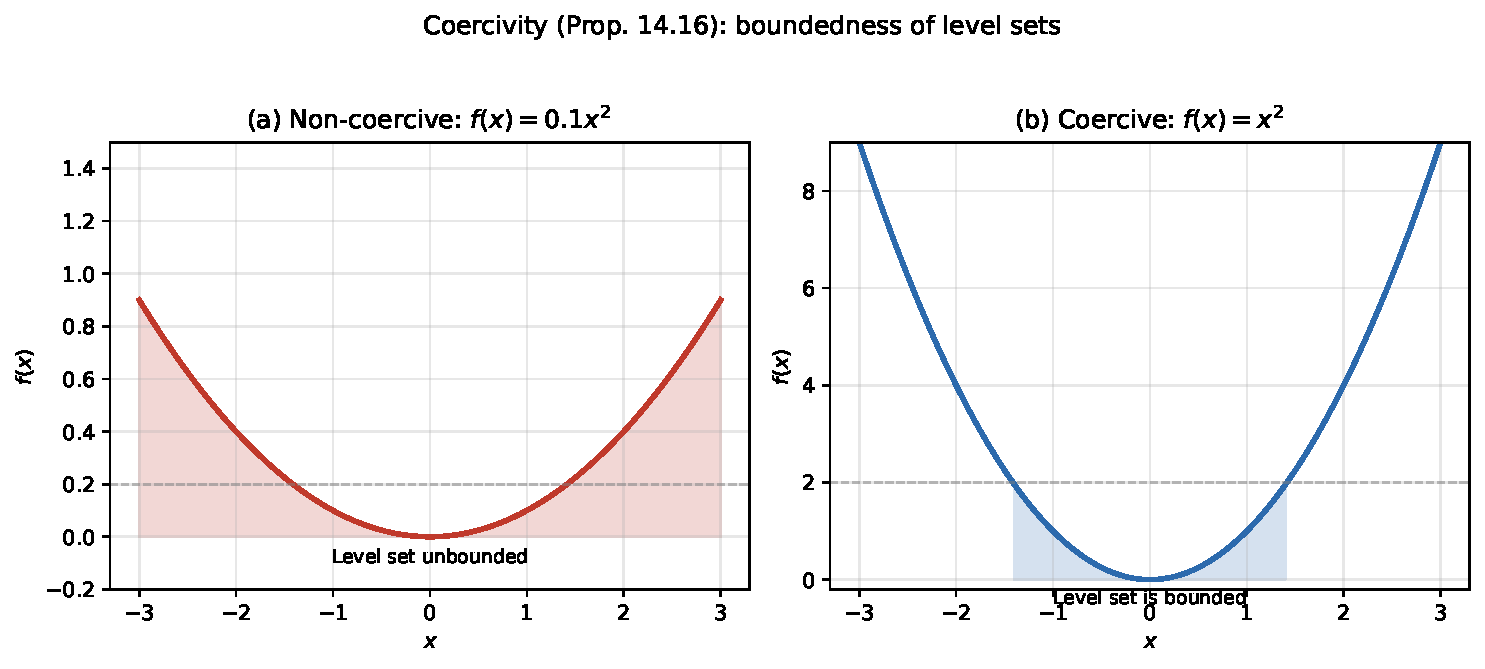
\includegraphics[width=0.95\textwidth]{fig_coercivity.pdf}
\end{frame}

% ━━━━━━━━━━━━━━━━━━━━━━━━━━━━━━━━━━━━━━━━━━━━━━━━━━━━━━━━━━━━━━━━━━━━━━━━━━━

\section{Conjugate of a Difference}

\begin{frame}{14.5: The Conjugate of a Difference}
  \vspace{-0.3cm}

  \begin{prop}[14.19]
    Let $g: \mathcal{H} \to \mathbb{R} \cup \{+\infty\}$ be proper, let $h \in \Gamma_0(\mathcal{H})$, and set:
    \[
      f(x) = \begin{cases}
        g(x) - h(x) & \text{if } x \in \dom g \\
        +\infty & \text{if } x \notin \dom g
      \end{cases}
    \]

    Then:
    \[
      (\forall u \in \mathcal{H}) \quad f^*(u) = \sup_{v \in \dom h^*} (g^*(u+v) - h^*(v))
    \]
  \end{prop}
\end{frame}

\begin{frame}{Toland-Singer Formula}
  \vspace{-0.3cm}

  \begin{cor}[14.20: Toland-Singer]
    Let $g, h \in \Gamma_0(\mathcal{H})$. Then:
    \[
      \inf_{x \in \dom g} (g(x) - h(x)) = \inf_{v \in \dom h^*} (h^*(v) - g^*(v))
    \]
  \end{cor}

  \vspace{0.3cm}

  \textbf{Key insight:} The Toland-Singer formula provides a dual problem for minimizing
  differences of convex functions. This is crucial for solving optimization problems of the form:
  \[
    \min_x (g(x) - h(x))
  \]
  by reformulating as a dual maximization problem.
\end{frame}

% ━━━━━━━━━━━━━━━━━━━━━━━━━━━━━━━━━━━━━━━━━━━━━━━━━━━━━━━━━━━━━━━━━━━━━━━━━━━

\section{Numerical Examples}

\begin{frame}[fragile]{Python Implementation: Soft Thresholding}
  \vspace{-0.3cm}

  \begin{lstlisting}
import numpy as np
import scipy.optimize as opt

# Example 14.5: Soft thresholding (proximal operator of f = rho*||x||)
def soft_threshold(x, rho):
    """Compute Prox_f(x) where f(x) = rho * ||x||"""
    return np.sign(x) * np.maximum(np.abs(x) - rho, 0)

def moreau_envelope(x, rho):
    """Compute ^1 f(x) = generalized Huber function"""
    abs_x = np.abs(x)
    return np.where(abs_x > rho,
                    rho * abs_x - rho**2 / 2,
                    abs_x**2 / 2)

# Verify Moreau decomposition: f = Prox_f + Moreau_envelope
rho = 1.5
x = np.linspace(-4, 4, 100)
f = rho * np.abs(x)
prox = soft_threshold(x, rho)
envelope = moreau_envelope(x, rho)

# Check: f(Prox_f(x)) + envelope(x) = (1/2) ||x||^2
verification = f[np.abs(prox) > 0] + envelope[np.abs(prox) > 0]
  \end{lstlisting}
\end{frame}

\begin{frame}[fragile]{Proximal Average Computation}
  \vspace{-0.3cm}

  \begin{lstlisting}
from scipy.optimize import minimize_scalar

def proximal_average(f, g, x, max_iter=1000):
    """
    Compute pav(f,g)(x) from Definition 14.6
    pav(f,g)(x) = (1/2) * min_{y,z: y+z=2x}
                  [f(y) + g(z) + (1/4)||y-z||^2]
    """
    def objective(y):
        z = 2*x - y
        return f(y) + g(z) + 0.25 * np.linalg.norm(y - z)**2

    result = minimize_scalar(objective, bounds=(x-10, x+10),
                           method='bounded',
                           options={'xatol': 1e-10})
    return 0.5 * result.fun

# Example: pav of f(x) = x^2/2 and g(x) = |x|
f = lambda y: 0.5 * y**2
g = lambda z: np.abs(z)

x_vals = np.linspace(-2, 2, 50)
pav_vals = [proximal_average(f, g, x) for x in x_vals]
  \end{lstlisting}
\end{frame}

\begin{frame}[fragile]{Coercivity Check}
  \vspace{-0.3cm}

  \begin{lstlisting}
def is_coercive(f, x_test=None):
    """
    Check coercivity by verifying boundedness of level sets
    (Theorem 14.16): f is coercive iff all lev_{<=c}(f) are bounded
    """
    if x_test is None:
        x_test = np.logspace(0, 3, 100)  # Test x from 1 to 1000

    # Check if f(x)/||x|| -> infinity as ||x|| -> infinity
    ratios = []
    for x in x_test:
        x_vec = np.ones(10) * x  # Test in R^10
        f_val = f(x_vec)
        x_norm = np.linalg.norm(x_vec)
        if x_norm > 0:
            ratios.append(f_val / x_norm)

    return min(ratios) > 0  # Coercive if min ratio > 0

# Example: f(x) = x^2 is coercive
f_coercive = lambda x: np.sum(x**2)

# Example: f(x) = 0.1*x^2 grows slowly, not coercive
f_noncoercive = lambda x: 0.1 * np.sum(x**2)

print(f"f(x)=x^2 coercive: {is_coercive(f_coercive)}")
print(f"f(x)=0.1*x^2 coercive: {is_coercive(f_noncoercive)}")
  \end{lstlisting}
\end{frame}

\begin{frame}[fragile]{Strongly Convex Conjugates}
  \vspace{-0.3cm}

  \begin{lstlisting}
def strongly_convex_conjugate_example():
    """
    Proposition 14.2 & Theorem 14.3:
    If f is strongly convex, then f^* is strictly convex.
    """
    gamma = 1.0
    q = lambda x: 0.5 * np.linalg.norm(x)**2  # q(x) = (1/2)||x||^2

    # Example: f(x) = (gamma/2)*||x||^2, self-conjugate
    f = lambda x: (gamma / 2) * np.linalg.norm(x)**2
    f_star = lambda u: (0.5 / gamma) * np.linalg.norm(u)**2

    # Proximal operator (Theorem 14.3 part ii)
    def prox_f(x, step=1.0):
        return x / (1.0 + gamma * step)

    # Verify: f^* - (1/gamma)*q is convex
    # For this example, f^* = (1/2*gamma)*||.||^2, so
    # f^* - (1/gamma)*q = (1/2*gamma - 1/gamma)*||.||^2
    #                   = -(1/2*gamma)*||.||^2, still convex!

    x_test = np.linspace(-2, 2, 100)

    return f, f_star, prox_f
  \end{lstlisting}
\end{frame}

\begin{frame}{Strongly Convex Functions Visualization}
  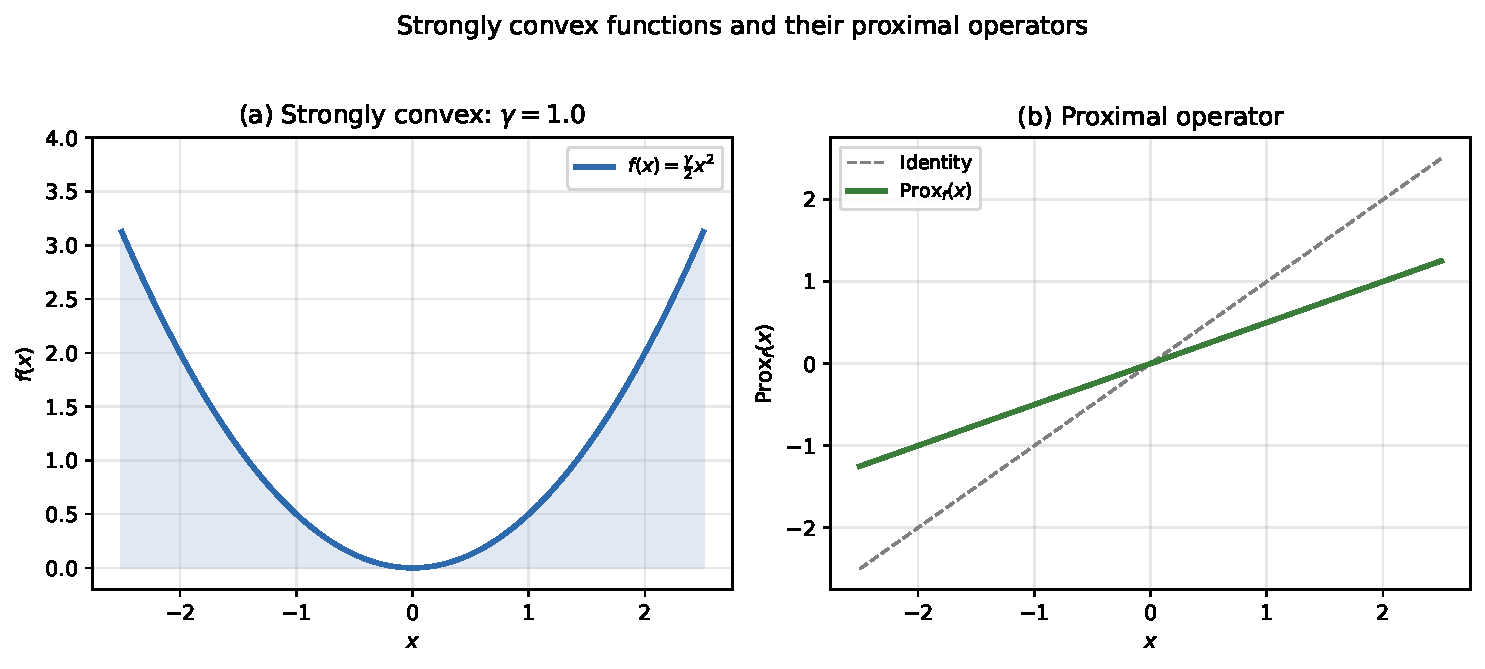
\includegraphics[width=0.95\textwidth]{fig_strongly_convex.pdf}
\end{frame}

% ━━━━━━━━━━━━━━━━━━━━━━━━━━━━━━━━━━━━━━━━━━━━━━━━━━━━━━━━━━━━━━━━━━━━━━━━━━━

\section{Summary}

\begin{frame}{Chapter 14: Key Takeaways}
  \vspace{-0.3cm}

  \begin{enumerate}
    \item \textbf{Strongly Convex Conjugates} (14.1-14.2):
      \begin{itemize}
        \item Strong convexity of $f^*$ characterized by convexity of $\gamma q - f$
        \item Theorem 14.3 connects proximal operators and conjugates
      \end{itemize}

    \item \textbf{Proximal Average} (14.2):
      \begin{itemize}
        \item Midpoint between convex functions, sandwiched between $(f+g)/2$ and lower bound
        \item Self-dual structure: $(\pav(f,g))^* = \pav(f^*, g^*)$
        \item Proximal operator: $\Prox_{\pav(f,g)} = \frac{1}{2}\Prox_f + \frac{1}{2}\Prox_g$
      \end{itemize}

    \item \textbf{Positively Homogeneous Functions} (14.3):
      \begin{itemize}
        \item Characterized as support functions of closed convex sets
        \item Connection to Minkowski gauge
      \end{itemize}

    \item \textbf{Coercivity} (14.4):
      \begin{itemize}
        \item Functions with bounded level sets
        \item Moreau-Rockafellar theorem: $u \in \text{int} \dom f^* \Leftrightarrow$ coercivity
      \end{itemize}

    \item \textbf{Conjugate of Difference} (14.5):
      \begin{itemize}
        \item Toland-Singer formula for dual optimization
      \end{itemize}
  \end{enumerate}
\end{frame}

\begin{frame}{Further Reading}
  \vspace{-0.3cm}

  \begin{itemize}
    \item \textbf{Related Chapters:}
      \begin{itemize}
        \item Chapter 12: Duality and conjugacy fundamentals
        \item Chapter 13: Subdifferentials and proximity operators
        \item Chapter 15: Fenchel-Rockafellar duality
      \end{itemize}

    \item \textbf{Key Authors \& References:}
      \begin{itemize}
        \item J.J. Moreau: Proximal analysis and decomposition theorems
        \item R.T. Rockafellar: Convex analysis and duality theory
        \item I. Singer, P. Tseng, H. Bauschke: Further conjugacy results
      \end{itemize}

    \item \textbf{Applications:}
      \begin{itemize}
        \item Soft thresholding in signal processing and compressed sensing
        \item Proximal splitting algorithms (Douglas-Rachford, ADMM)
        \item Machine learning: regularized convex optimization
      \end{itemize}
  \end{itemize}
\end{frame}

\end{document}
